\chapter{GPSa and beyond}
\label{ch:skeletons}

The skeletons described in this chapter are automatically generated if the specification passes the \gls{zdra} check. Section \ref{sec:zdra2gen} describes the general proof skeleton. Which uses the graphs generated in the \gls{zdra} to provide the order the instaces should go to into any theorem prover. Section \ref{sec:gpsa2isa} then explains how a general proof skeleton can be automatically translated into a skeleton in Isabelle format automatically. In section \ref{sec:isa2ful} we describe how the Isabelle Skeleton can be used to fully prove a formal specification which requires two steps, the first is an automatic step to fill in the Isabelle skeleton and the final step is up to the user to prove the lemma's and properties of the specification.

\section{From ZDRa to General Proof Sketch}
\label{sec:zdra2gen}

When checking for ZDRa correctness the program adds all the annotated chunks into a dependency graph and a GoTo graph. Both these graphs are directed graphs.

We then run an algorithm on the GoTo graph to generate a proof skeleton. Figure \ref{fig:code} shows part of the code in generating this proof sketch.

\begin{itemize}
\item \textit{allnodes}, is a set of all the instances labelled by the user of a specification in ZDRa.

\item \textit{fromnodes}, is a set containing all the nodes which are dependent on another instance.

\item \textit{tonodes}, is a set containing all the nodes which have some other nodes dependent on them.
\end{itemize}

\begin{figure}[H]
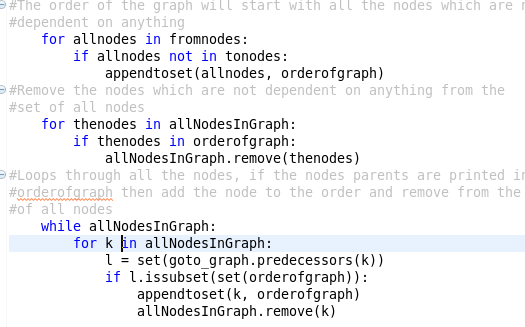
\includegraphics[scale=0.5]{Figures/skeleton/code.png}
\caption{Part of the algorithm to create a proof sketch.}
\label{fig:code}
\end{figure}

\subsection{Creating the Graph}

Here we show how a Proof skeleton is calculated using the Goto graph created when running the ZDRa check on a specification.

\begin{figure}[H]
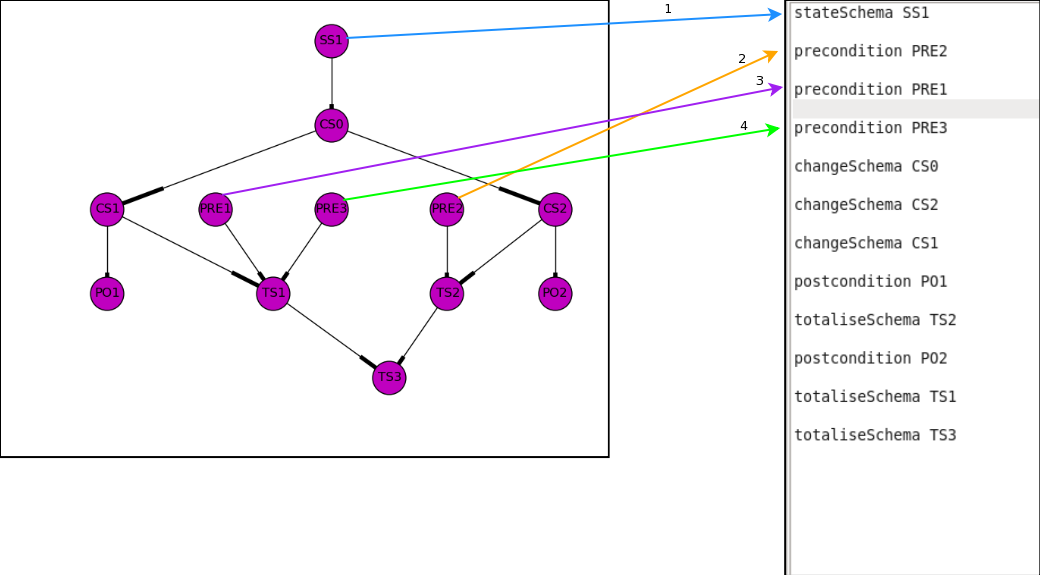
\includegraphics[scale=0.3]{Figures/skeleton/1.png}
\caption{GoTo graph and proof skeleton of vending machine step 1.}
\label{fig:1}
\end{figure}

First of all the program looks at all the nodes of the GoTo graph and prints out all the nodes which are not dependent on anything. That is, they may have successors but they have no predecessors, they do not use or need anything else and can stand by themselves. These nodes can be printed in any order, so in diagram \ref{fig:1} we see that we have SS1, PRE1 PRE2 and PRE3 all printed.

\begin{figure}[H]
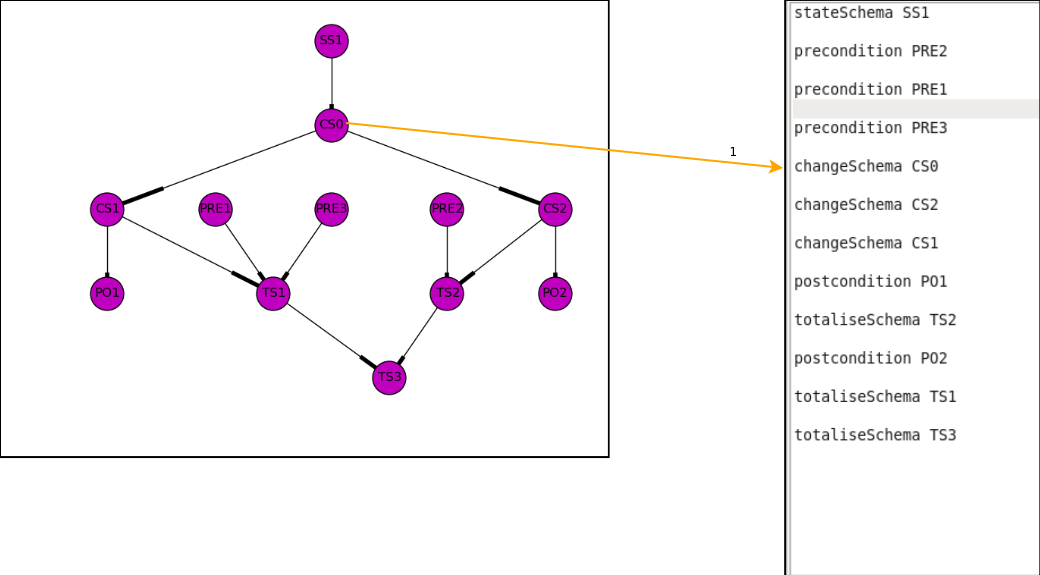
\includegraphics[scale=0.3]{Figures/skeleton/2.png}
\caption{GoTo graph and proof skeleton of vending machine step 2.}
\label{fig:2}
\end{figure}

The next part of the algorithm checks whether there exists a node in the GoTo graph where all of its parents are printed out in the proof skeleton. Figure \ref{fig:2} shows that the next node to be in the proof skeleton is CS0. 

\begin{figure}[H]
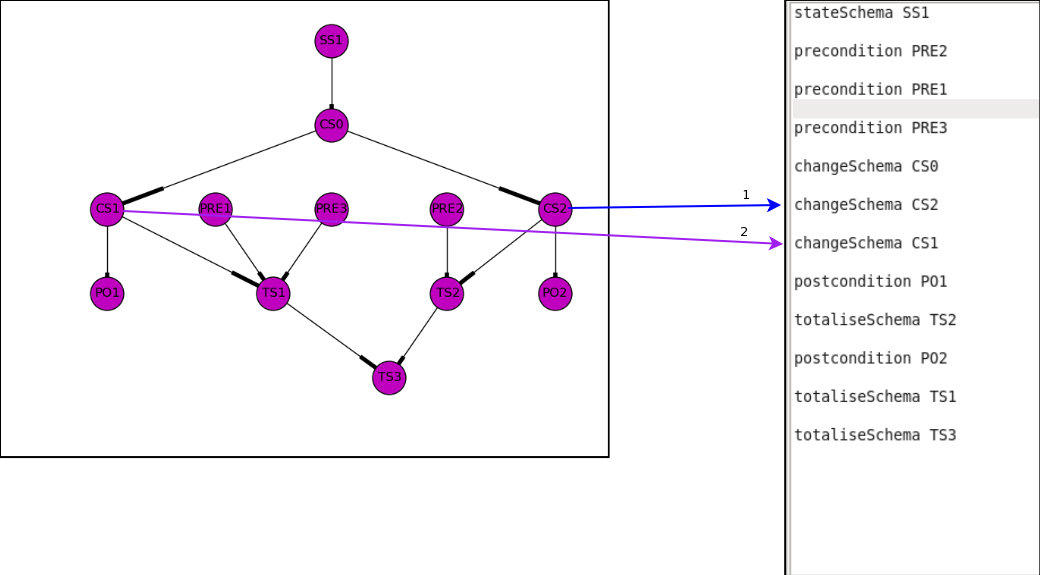
\includegraphics[scale=0.3]{Figures/skeleton/3.png}
\caption{GoTo graph and proof skeleton of vending machine step 3.}
\label{fig:3}
\end{figure}

The next part we see that after CS0 is added to the proof skeleton then both CS1, and CS2 can be added. This is shown in figure \ref{fig:3}.

\begin{figure}[H]
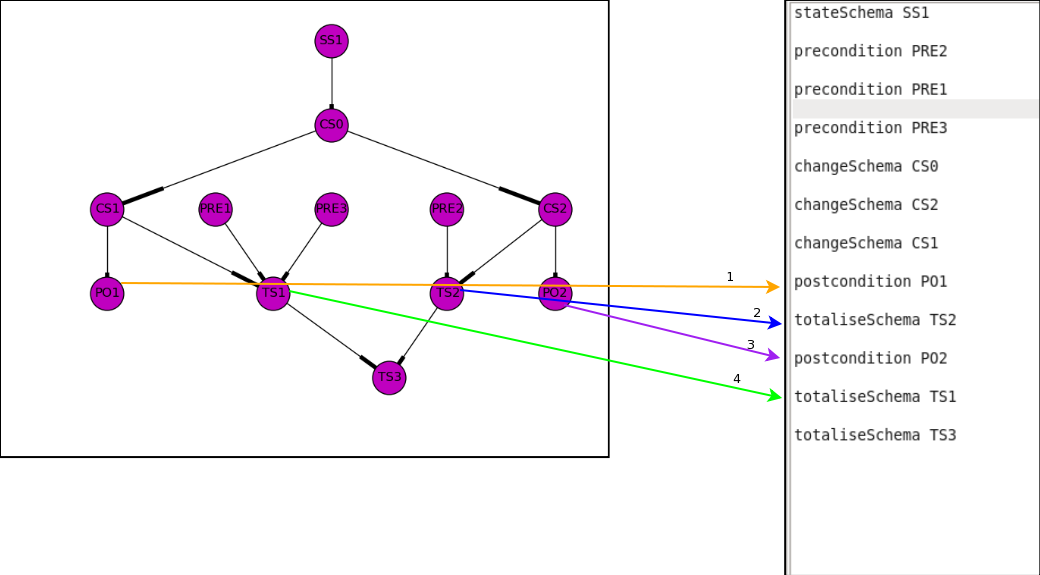
\includegraphics[scale=0.3]{Figures/skeleton/4.png}
\caption{GoTo graph and proof skeleton of vending machine step 4.}
\label{fig:4}
\end{figure}

Figure \ref{fig:4} shows the next stage of adding nodes to the Proof Skeleton. Since CS1 and CS2 are now added to the proof skeleton then the next row of nodes can be added. Since PO1 only had one parent (CS1) it is added first, PO2 also had one parent (CS2) it is added second. The others had more parents which are already in the proof sketch so they are added next randomly.

\begin{figure}[H]
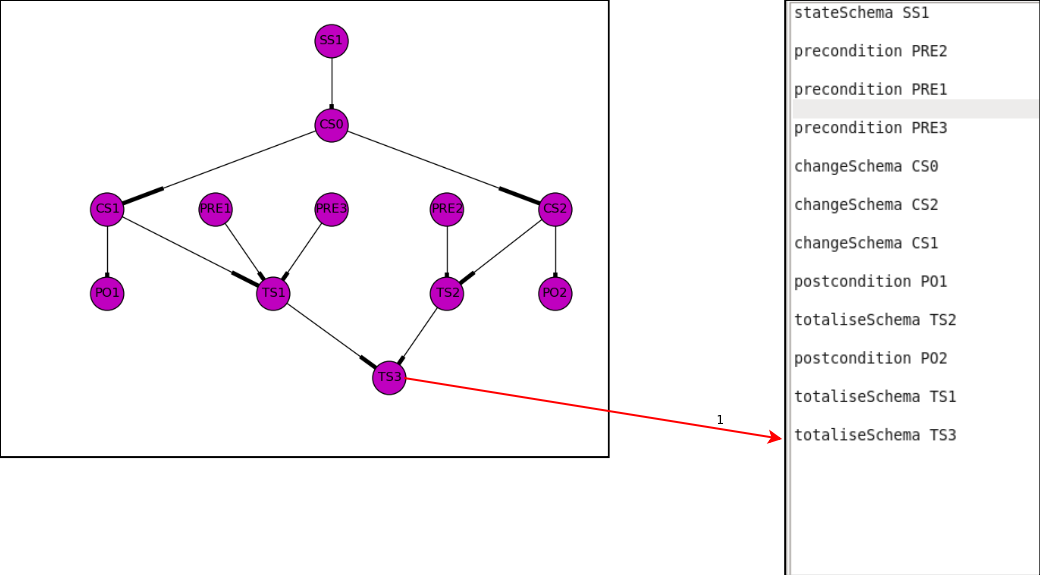
\includegraphics[scale=0.3]{Figures/skeleton/5.png}
\caption{GoTo graph and proof skeleton of vending machine step 5.}
\label{fig:5}
\end{figure}

We come to the final stage of the dependency graph, when all the nodes are in the dependency graph except for one which is added to the end.

\section{General Proof Sketch aspect into Isabelle Skeleton}
\label{sec:gpsa2isa}

When translating from the \gls{zdra} annotated specification to the Isabelle skeleton, the syntax needed to be changed in order for the specification to parse through Isabelle. In this section we outline how the Z specification is translated into Isabelle.

If the user has labelled a theory in the specification (T\#) then that will begin writing an Isabelle skeleton.

For example if we had an empty specification and named it a then the program will create an empty Isabelle skeleton such as:

\begin{verbatim}
theory gpsa_a
imports
main
begin
end
\end{verbatim}

If the user labels a schema `\texttt{SS1}' meaning the state schema of the specification then that in Isabelle becomes a `\texttt{record}' and a `\texttt{locale}' is created. Using our example of specifcation named `\texttt{a}' we get the following (after the premuable descibed before):
\begin{verbatim}
record SS1 =
(*DECLARATIONS*)
locale a =
fixes (*GLOBAL DECLARATIONS*)
assumes SI#
begin
end
end
\end{verbatim}

If there are no state invarients in the state schema at this point then there is no `\texttt{assumes SI\#}') line.

All other schemas including changeSchemas, outputSchemas, preconditions that are schemas, post conditions that are schemas and all other state schema become definitions in the Isabelle skeleton.
So for example if we have the following schema writte in \gls{zdra}
\begin{verbatim}
\draschema{CS1}{
\begin{schema}{b}
someDeclaration
\where
\draline{PO1}{someExpression}
\end{schema}}
\end{verbatim}

Then when translating into the Isabelle skeleton it becomes:
\begin{verbatim}
definition CS1 ::
"(*CS1_TYPES*) => bool"
where
"CS1 (*CS1_VARIABLES*) == PO1"
\end{verbatim}

At this stage it doesn't matter what the declarations and expressions are as they get filled in at the next stage. The Isabelle skeleton only uses the \gls{zdra} labels to be created.

Totalising schemas, written either horizontally or vertically in a specification become lemmas when translating into the Isabelle skeleton. If the use wishes to prove the correctness of certain safety aspects (such as the specification is total) then they can label the schema's the the annotation \verb|\draline{TS#}|. For example if we have the following totalisingSchema:

\verb|\draline{TS1}{someSchema == someExpression}|

This would translate to the Isabelle skeleton as:

\begin{verbatim}
lemma TS1:
"(*TS1_EXPRESSION*)"
sorry
\end{verbatim}

Again, at this stage it doesn't matter what the expression is. We put `\texttt{sorry}' at the end of the lemma as this lemma will need to be proved  by the user in the final stage.

\subsection{Benefits}

The Isabelle skeleton allows for incomplete specifications to also be automated into a half-baked proof. This way the user can have a general outline for their specification and fill in the missing information directly into the Isabelle skeleton at a later stage. For this reason it is good to have an Isabelle skeleton before the full filled in half-baked proof.

\section{ZCGa specification to Fill in the Isabelle Skeleton}

Since translating using ZMathLang to translate Z specifications into an Isabelle skeleton can even been done on incomplete specifications, it is important to note that if some missing information is missing e.g. a declaration, expression etc then the comments of where these should go will not be changed. 
For example if we have the line \verb|"(*CS1_TYPES*) => bool"| in the skeleton and the schema CS1 has no declarations yet then the line will not be changed, and it is up to the user to input the variables and the types of that definition.

It is important to note that all the \gls{zcga} annotations at this stage disappear as the labelled information is automatically put into Isabelle syntax.

\subsection{Z Types and FreeTypes}

The program which fills in the Isabelle skeleton goes through the entire specification and adds any Z declared types and freetypes before the record. For example, if a specification has the following:
\begin{verbatim}
\begin{zed}
[STUDENT]
\end{zed}
\end{verbatim}

Then the line \verb|typedecl STUDENT| will be added after the first begin in the skeleton.

If the specification had the following freetype:
\begin{verbatim}
\begin{zed} 
REPORT ::= ok | already\_known | not\_known
\end{zed}
\end{verbatim}

Then again, in the same place as the Z-Types the line
\begin{verbatim}
datatype  REPORT = ok | already_known | not_known
\end{verbatim}
is added to the skeleton.

\subsection{Declarations}

In Isabelle the types and variables are added speratly. For insance if we had the following schema:

\begin{verbatim}
\draschema{OS1}{
\begin{schema}{ab}
d: \power COLOUR
c: COLOUR
\where
\draline{PO1}{c \in d}
\end{schema}}
\end{verbatim}

Then the Isabelle skeleton for this schema will be as follows:

\begin{verbatim}
definition OS1 ::
"(*OS1_TYPES*) => bool"
where
"OS1 (*OS1_VARIABLES*) == (PO1)"
\end{verbatim}

Since we have two declarations, the filling in program would change the definition in the skeleton as follows:

\begin{verbatim}
definition ab ::
"COLOUR set => COLOUR => bool"
where
"ab d c == (c \<in> d)"
\end{verbatim}

Therefore, from the declarations, the types replace the line \verb|(*OS1_TYPES*)| and the variables replace the line \verb|(*OS1_VARIABLES*)|.

\subsection{Expressions}

Since the majority of the syntax for expressions is very similar to the syntax in Isabelle, the expressions are put in directly with minor changes. The expressions replace the \gls{zdra} labellings.

Using our previous example shown in the last section, we have the schema `\texttt{ab}', in the skeleton we have a label `\texttt{PO1}' which is then replaced by the expression \verb|c \<in> d|. Note this expression is very similar to the expression in \LaTeX{} \verb|c \in d| apart from the symbol \verb|\in| becomes \verb|\<in>|. Table \ref{tab:latextoisabelle} shows the rest of these automatic changes of the syntax made from \LaTeX{} to Isabelle.

{\def\arraystretch{0.5}\tabcolsep=0.5pt
\begin{longtable}[H]{|c | c | c |}
\hline
\textbf{Syntax in Z} & \textbf{Syntax in \LaTeX} & \textbf{Syntax in Isabelle} \\
\hline
$\{...\}$ & \verb|\{...\}| & \verb|{...}|\\
$\limg...\rimg$ & \verb|\limg...\rimg| & \verb|\<lparr>...\<rparr>| \\
$\langle...\rangle$ & \verb|\langle...\rangle| & \verb|\<langle>...\<rangle>| \\
$\# $ A & \verb|\#| & \verb|card| \textit{if A is set}, \\
& & \verb|length| \textit{if A is list} \\
$\cup $ & \verb|\cup| & \verb|\<union>| \\
$\cap$ & \verb|\cap| & \verb|\<inter>| \\
$\cross$ & \verb|\cross| & \verb|\<times>| \\
$\setminus$ & \verb|\setminus| & \verb|-| \\
$\geq$ & \verb|\geq| & \verb|\<ge>| \\
$\leq$ & \verb|\leq| & \verb|\<le>| \\
$\lhd$ & \verb|\lhd| & \verb|\<lhd>| \\
$\rhd$ & \verb|\rhd| & \verb|\<rhd>| \\
$\nrres$ & \verb|\nrres| & \verb|\<unlhd>| \\
$\ndres$ & \verb|\ndres| & \verb|\<unrhd>| \\
$\implies$ & \verb|\implies| & \verb|\<Longrightarrow>| \\
$\iff$ & \verb|\iff| & \verb|\<Longleftrightarrow>| \\
$\notin$ & \verb|\notin| & \verb|\<notin>| \\
$\in$ & \verb|\in| & \verb|\<in>| \\
$\subset$ & \verb|\subset| & \verb|\<subset>| \\
$\subseteq$ & \verb|\subseteq| & \verb|\<subseteq>| \\
$\land$ & \verb|\land| & \verb|\<and>| \\
$\lor$ & \verb|\lor| & \verb|\<or>| \\
$\lnot$ & \verb|\lnot| & \verb|\<not>| \\
$\neq$ & \verb|\neq| & \verb|\<noteq>| \\
$a \mapsto b$ & \verb|a \mapsto b| & \verb|(a,b)| \\
$\power A$ & \verb|\power A| & \verb|A set| \\
$\nat$ & \verb|\nat| & \verb|nat| \\
$\nat_1$ & \verb|\nat_1| & \verb|nat| \\
$\num$ & \verb|\num| & \verb|num| \\
$A \pfun B$ & \verb|A \pfun B| & \verb|(A * B) set| \\
$A \fun B$ & \verb|A \fun B| & \verb|(A * B) set| \\
$A \rel B$ & \verb|A \rel B| & \verb|(A * B) set| \\
$\seq A$ & \verb|\seq A| & \verb|A list| \\
$\iseq A$ & \verb|\iseq A| & \verb|A list| \\
$\seq_1 A$ & \verb|\iseq_1 A| & \verb|A list| \\
$\dom A$ & \verb|\dom A| & \verb|Domain A| \\
$\ran A$ & \verb|\ran A| & \verb|Range A| \\
$\exists$ & \verb|\exists| & \verb|\<exists>| \\
$\forall$ & \verb|\forall| & \verb|\<forall>| \\
$@$ & \verb|@| & \verb|\<bullet>| \\
$R\inv$ & \verb|R\inv| & \verb|\<R^-1>| \\
$R^{k}$ & \verb|R^{k}| & \verb|\<R^k>| \\
\hline
\caption{A table showing the symbols which are changed from Z specifications in \LaTeX{} to Isabelle.}
\label{tab:latextoisabelle}
\end{longtable}
}

Another part of the Z mathematical toolkit which we need to rewrite are the use of partial functions. In HOL all functions are total but there are ways to do certain proofs about partial functions \cite{Krauss08definingrecursive}. Therefore the variables which have a type as a partial function will are translated as a set of pairs. Any proofs to check for partial functions if needed can be done by the user in step 6 shown in figure \ref{fig:steps} but the details of these proofs are beyond the scope of this thesis.

\subsection{Schema Names}

The Names of the Schema are added to the skeleton by using the \gls{zdra} name. For example if the specification had the line \verb|\draschema{TS1}{\begin{schema}{ab}{..| then anywhere `\texttt{TS1}' is listed in the skeleton it will be converted to `\texttt{ab}'. This is done throughout the entire skeleton.

\section{Filled in Isabelle Skeleton to a Full Proof}
\label{sec:isa2ful}

The final step to get from a half-baked proof into a full proof is labelled as step 7 in Figure \ref{fig:steps}, this is also named fill in 2. Technically the specification the user automatically generates in fill in 1 is fully formalised in Isabelle if there are no other properties to be proved. If the specification is not fully formalised, using the half-baked proof generated in step 5, the user then adds any safety properties about the specification they wish to prove in the form of \emph{lemmas}. As the properties will be specific to the user and/or specification it is difficult to automate this step. Therefore some theorem prover knowledge may be required for step 6. Some of the automated theorem prover tools such as Sledgehammer \cite{sledgehammer} may be useful when proving the properties.

It is important to note that when proving the properties sometimes it is useful to unfold the definitions which have been automatically created from the specification.
For example figure \ref{fig:exampleproof} shows an example of a lemma automatically generated from the \gls{zdra} annotated specification (black) and the user input needed to prove this lemma (red). Notice that the user has deleted the word "\texttt{sorry}" which would have automatically come after the lemma. The user usually needs to unfold the definitions by applying the unfold rule to the definitions of the schemas. More information on proving these lemmas can be found in the Isabelle Manual \cite{isabelle} and is beyond the scope of this thesis.

\begin{center}
\begin{figure}[H]
\centering
\begin{footnotesize}
\begin{BVerbatim}[commandchars=+\[\]]
lemma pre_VM1: 
"(\<exists> stock' takings' cash_refunded bars_delivered.
VM1 cash_tendered stock takings stock' takings' cash_refunded bars_delivered)
\<longleftrightarrow> (0 < stock) \<and> (cash_tendered = price) \<and> 
(0 \<le> takings)"
[+color[red]apply (unfold VM1_def exact_cash_def some_stock_def VM_sale_def)]
[+color[red]apply auto]
[+color[red]done]
\end{BVerbatim}
\end{footnotesize}
\caption{\label{fig:exampleproof} An example of a proof completed by user input.}
\end{figure}
\end{center}

\section{Conclusion}
\label{sec:skeletonsConclusion}

This chapter described the final steps in computerising a formal specification into full proof. It has described how the \gls{zdra} program uses the GoTo graph to generate a general proof skeleton (step 2$\rightarrow$3 in figure \ref{fig:steps}), then it examples how the program uses the automatically generated general skeleton to  create an Isabelle skeleton. From the Isabelle skeleton the user can then automatically fill in the skeleton using the \gls{zcga} annoatated specification giving a \gls{half}. The last step would be to fill in any mising proofs in the \gls{half}, this is still a difficult step and may require some theorem prover knowledge however this part is difficult to automate as different system specifications have different properties users wish to prove, therefore tools such as sledgehammer \cite{sledgehammer} may be useful at this point.

In the next chapeter we demonstrate a full example of a specification being taken through all the steps of the ZMathLang framework.